\documentclass[11pt]{article}
\usepackage{geometry}                % See geometry.pdf to learn the layout options. There are lots.
\geometry{letterpaper}                   % ... or a4paper or a5paper or ... 
%\geometry{landscape}                % Activate for for rotated page geometry
%\usepackage[parfill]{parskip}    % Activate to begin paragraphs with an empty line rather than an indent
\usepackage{graphicx}
\usepackage{latexsym}
\usepackage{amsmath}
\usepackage{amssymb}
\usepackage{natbib}
\usepackage{subcaption}
\usepackage{hyperref}
\usepackage{enumerate}
\hypersetup{colorlinks = true, urlcolor = blue, citecolor =red}
\usepackage{tikz}
\usetikzlibrary{arrows,automata}

\DeclareMathOperator{\ELBO}{ELBO}
\DeclareMathOperator{\KL}{KL}
\DeclareMathOperator{\Cat}{Cat}
\DeclareMathOperator{\Dir}{Dir}

\newcommand{\itembrack}[1]{\ensuremath{\left[ #1 \right]}}
\newcommand{\angbrack}[1]{\ensuremath{\left\langle #1 \right\rangle}}

\title{Earley intersection}
\author{Wilker Aziz}
\date{}

\begin{document}
\maketitle


Earley parsers \citep{Earley:1970} can deal with arbitrary context-free grammars (CFGs), that is, they impose no constraints on:
\begin{itemize}
	\item left-recursion;
	\item length of right-hand side of rules;
	\item epsilon rules
\end{itemize}

We will be working with a generalised view of parsing corresponding to intersection between discrete (potentially infinite) sets \citep{BarHillel+1961,Billott+1989}. One set is finite-state, another set is context-free, and the result (the intersection) is also context-free. 
To draw a parallel with standard parsing, the FSA corresponds to the input sentence, the CFG corresponds to the grammar, the intersection corresponds to a parse forest (or chart).

This generalisation is interesting because when dealing with probability distributions over complex discrete spaces (such as those in parsing and hierarchical MT), it is convenient to be able to parse finite-state automata that can represent more than single sentences.

\section{FSA} 

An FSA is a $5$-tuple $A = \angbrack{\Sigma, Q, E, I, F}$ where
\begin{itemize}
	\item $\Sigma$ is a finite set of labels (e.g. words);
	\item $Q$ is a finite set of states;
	\item $E$ is a finite set of arcs;
	\item $I$ is a finite set of initial states;
	\item $F$ is a finite set of final/accepting states.
\end{itemize}
An arc is a tuple $\angbrack{q, x, s}$ with $(q, s) \in Q \times Q$ and $x \in \Sigma$.
An FSA defines a \emph{language} $L(A)$ which correspond to the set of sentences that is accepted by $A$.
A sentence $\mathbf x$ is accepted if there is a path from a state in $I$ (an initial state) to a state in $F$ (an accepting state) whose label sequence corresponds to $\mathbf x$. See Figure \ref{fig:fsa} for examples.

\begin{figure}\centering
\begin{subfigure}[t]{\textwidth}\centering
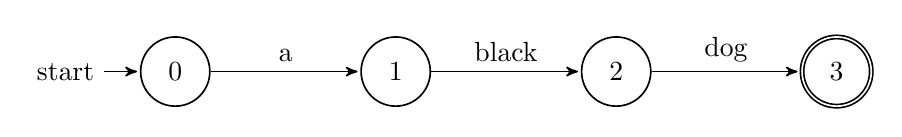
\begin{tikzpicture}[->,>=stealth',shorten >=1pt,auto,node distance=2.8cm,
                    semithick]
  %\tikzstyle{every state}=[fill=red,draw=none,text=white]

  \node[initial,state] (A)                    {$0$};
  \node[state]         (B) [right of=A] {$1$};
  \node[state]         (C) [right of=B] {$2$};
  \node[state,accepting]         (D) [right of=C] {$3$};
  \path (A) edge              node {a} (B)
        (B) edge              node {black} (C)
        (C) edge              node {dog} (D);
\end{tikzpicture}
\caption{\label{fig:s1}A \emph{linear-chain} FSA is convenient for representing single sentences. Accepting states are denoted by double circles. In this case $L(A) = \{\text{``a black dog''}\}$.}
\end{subfigure}
\begin{subfigure}[t]{\textwidth}\centering
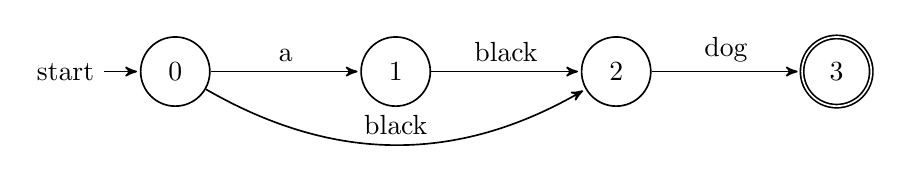
\begin{tikzpicture}[->,>=stealth',shorten >=1pt,auto,node distance=2.8cm,
                    semithick]
  %\tikzstyle{every state}=[fill=red,draw=none,text=white]

  \node[initial,state] (A)                    {$0$};
  \node[state]         (B) [right of=A] {$1$};
  \node[state]         (C) [right of=B] {$2$};
  \node[state,accepting]         (D) [right of=C] {$3$};
  \path (A) edge              node {a} (B)
        (A) edge [bend right]  node {black} (C)
        (B) edge              node {black} (C)
        (C) edge              node {dog} (D);
\end{tikzpicture}
\caption{\label{fig:s2}An FSA can define larger sets, for example, in this case $L(A) = \{\text{``a black dog'', ``black dog''}\}$.}
\end{subfigure}
\begin{subfigure}[t]{\textwidth}\centering
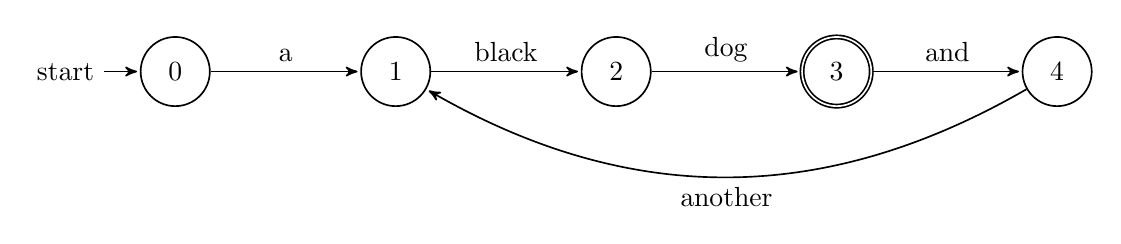
\begin{tikzpicture}[->,>=stealth',shorten >=1pt,auto,node distance=2.8cm,
                    semithick]
  %\tikzstyle{every state}=[fill=red,draw=none,text=white]

  \node[initial,state] (A)                    {$0$};
  \node[state]         (B) [right of=A] {$1$};
  \node[state]         (C) [right of=B] {$2$};
  \node[state,accepting]         (D) [right of=C] {$3$};
  \node[state]         (E) [right of=D] {$4$};
  \path (A) edge              node {a} (B)
        (B) edge              node {black} (C)
        (C) edge              node {dog} (D)
        (D) edge              node {and} (E)
        (E) edge [bend left] node {another} (B);
\end{tikzpicture}
\caption{\label{fig:sinf}An FSA can also definite infinitely large sets, for example, in this case $L(A)$ contains ``a black dog'' and infinitely many sentences made of ``a black dog'' concatenated with an arbitrary number of copies of ``and another black dog''.}
\end{subfigure}
\caption{\label{fig:fsa}Example of FSAs.}
\end{figure}





\section{CFG}


A CFG is a $4$-tuple $G = \angbrack{\Sigma, N, S, R}$ where
\begin{itemize}
	\item $\Sigma$ is a finite set of terminal symbols (e.g. words);
	\item $N$ is a finite set of nonterminal symbols (e.g. variables);
	\item $S \in N$ is a distinguished \emph{start} symbol;
	\item $R$ is a finite set of context-free rules/productions.
\end{itemize}
A rule has the form $X \rightarrow \alpha$ where $X \in N$ (the rule's \emph{left-hand side}---LHS) and $\alpha \in (\Sigma \cup N)^*$ (the rule's \emph{right-hand side}---RHS).
In other words, the rule's LHS is a single variable and the rule's RHS is a (possibly empty) sequence of terminal and nonterminal symbols.\footnote{An empty RHS is denoted by an empty string ($\epsilon$), for example, $X \rightarrow \epsilon$, we also call such rules \emph{epsilon rules}.}



\begin{figure}\centering
	\begin{subfigure}[b]{0.4\textwidth}\centering
        \begin{tabular}{l l l}
	        $S$ & $\rightarrow$ & $\epsilon$ \\
			$S$ & $\rightarrow$ & $X$ \\
			$X$ & $\rightarrow$ & $X ~ X$ \\
			$X$ & $\rightarrow$ & $a$ \\
		\end{tabular}
        \caption{\label{fig:g1} Set of rules of $G$.}
    \end{subfigure}
    ~
    \begin{subfigure}[b]{0.4\textwidth}\centering
		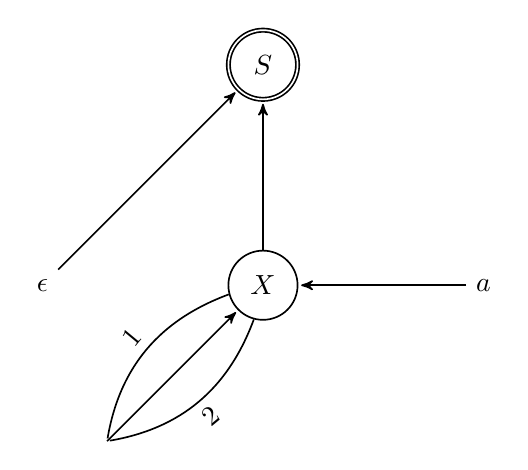
\begin{tikzpicture}[->,>=stealth',shorten >=1pt,auto,node distance=2.8cm,
		                    semithick]
		  %\tikzstyle{every state}=[fill=red,draw=none,text=white]
		
		  \node[state,accepting] (S)                    {$S$};  
		  \node[state]         (X) [below of=S] {$X$};
		  \coordinate[below left of=X] (p1);
		  \node[]         (a) [right of=X] {$a$};
		  \node[]         (eps) [left of=X] {$\epsilon$};
		  \path (X) edge (S)
		        (X) edge [-, bend right] node [pos=0.5, sloped, above]{1} (p1)
		        (X) edge [-, bend left]             node [pos=0.5, sloped, below]{2} (p1)
		        (p1) edge (X)
		        (a) edge (X)
		        (eps) edge (S);
		\end{tikzpicture}
		\caption{\label{fig:hg1} A graphical representation (a cyclic hypergraph) for the simple CFG in \ref{fig:g1}. The start symbol is denoted with double circles.}
	\end{subfigure}
	\caption{\label{fig:g1} A simple CFG: terminals are represented by lowercase letters. $L(G)$ contains the empty sentence and sentences made of arbitrarily many copies of ``a''.}
\end{figure}

\section{Earley intersection}

Our version of Earley intersection \citep{Dyer+2008:WLT,Dyer:2010:Bitext} will take an $\epsilon$-free FSA $A = \angbrack{\Sigma, Q, E, I, F}$ and an arbitrary CFG $G = \angbrack{\Sigma, N, S, R}$ and compute another CFG $G' = \angbrack{\Sigma, N', S', R'}$ such that $L(G') = L(A) \cap L(G)$.

In this presentation we will make use of deductive systems, thus we start by defining our item form
\begin{equation}
\itembrack{q, X \rightarrow \alpha_\blacksquare \bullet \beta_\square, r}
\end{equation}
where
\begin{itemize}
	\item $q$ and $r$ are states in $Q$: together they state that this item concerns all paths in $A$ from $q$ to $r$; 
	\item $X \rightarrow \alpha ~ \beta$ is a rule in $R$: note that $\alpha$ and $\beta$ are possibly empty sequences of terminals and nonterminals;
	\item $\bullet$ represents how far down the rule's RHS the algorithm has progressed, in particular, it states that the first part of the rule ($\alpha$) has already been intersected with FSA states, and that the second part ($\beta$) is yet to be dealt with;
	\item $\blacksquare$ is a shorthand for the FSA states that have already been intersected (in dealing with the symbols in $\alpha$);
	\item $\square$ is a there just to remind us that we still need to intersect the symbols in $\beta$ with FSA states.
\end{itemize}
For a concrete example, consider the FSA in Figure \ref{fig:s1} and the following fragment of a grammar
\begin{center}
\begin{tabular}{l l l}
$S$ & $\rightarrow$ & $NP$ \\
$S$ & $\rightarrow$ & $NP ~ VP$ \\
$NP$ & $\rightarrow$ & $NN$ \\
$NP$ & $\rightarrow$ & $DT ~ NN$ \\
$NP$ & $\rightarrow$ & $DT ~ JJ ~ NN$ \\
$DT$ & $\rightarrow$ & $\text{the}$ \\
$JJ$ & $\rightarrow$ & $\text{black}$ \\
$NN$ & $\rightarrow$ & $\text{dog}$ \\
\end{tabular}
\end{center}
then the item
$$\itembrack{0, NP \rightarrow DT_{0,1} ~ JJ_{1,2} \bullet NN, 2}$$
states that we have intersected paths from $0$ to $2$ in the automaton and this has allowed us to progress along the RHS of rule $NP \rightarrow DT ~ JJ ~ NN$ all the way to just before the last symbol ($NN$). We can interpret this as: every path from $0$ to $2$ in $A$ corresponds to an $NP$ missing an $NN$.
Can you extrapolate this to the case where between $0$ and $2$ we have multiple paths?

\noindent\textsc{Note on terminology} ~ in parsing literature the subscripts in the symbols of the item correspond to \emph{spans} and storing the in the item corresponds to keeping \emph{back-pointers}.


Now we are ready to present a complete intersection algorithm

\begin{align}
\text{Item form} &\quad  \itembrack{q, X \rightarrow \alpha_\blacksquare \bullet \beta_\square, r} & (q,r) \in Q\times Q \\
 & & X \rightarrow \alpha \beta \in R \nonumber \\
 & & \blacksquare \in Q^* \nonumber \\
\text{Axioms} &\quad \frac{}{\itembrack{q, S' \rightarrow \bullet S_\square}, q} & q \in I\\
\text{Goal} &\quad \itembrack{q, S' \rightarrow S_\blacksquare \bullet, r} & q \in I \text{ and } r \in F\\
\text{Predict} &\quad \frac{\itembrack{q, X \rightarrow \alpha_\blacksquare \bullet Y_\square \beta_\square, r}}{\itembrack{r, Y \rightarrow \bullet \gamma_\square, r}} & Y \rightarrow \gamma \in R \\
\Sigma\text{-Scan} &\quad \frac{\itembrack{q, X \rightarrow \alpha_\blacksquare \bullet x \beta_\square, r}}{\itembrack{q, X \rightarrow \alpha_\blacksquare x \bullet \beta_\square, s}} & x \neq \epsilon \text{ and } \angbrack{r, x, s} \in E \\
\epsilon\text{-Scan} &\quad \frac{\itembrack{q, X \rightarrow \alpha_\blacksquare \bullet \epsilon \beta_\square, r}}{\itembrack{q, X \rightarrow \alpha_\blacksquare \epsilon \bullet \beta_\square, r}} & \\
\text{Complete} &\quad \frac{\itembrack{q, X \rightarrow \alpha_\blacksquare \bullet Y_\square \beta_\square, r} ~ \itembrack{r, Y \rightarrow \gamma_\blacksquare \bullet, s}}{\itembrack{q, X \rightarrow \alpha_\blacksquare Y_{r,s} \bullet \beta_\square, s}}
\end{align}


\paragraph{Axioms} state that we can intersect sentences generated by the start symbol of $G$ as long as they project onto paths in $A$ that start from one of $A$'s initial states. We also introduce a new symbol $S'$ which will be the start symbol of the intersection $G'$.

\paragraph{Goal} is to have all derivations from $S$ project paths from an initial state of $A$ to a final state of $A$ (this is basically the condition that a sentence in the intersection must be in the language of $A$ and in the language of $G$).

\paragraph{Predict} introduces new items in the program by predicting that we will be able to intersect a rule $Y \rightarrow \gamma$ with paths from $r \in Q$.

\paragraph{Scan} deals separately with actual terminals and the empty string. The first variant simply moves the dot along the terminal if that terminal labels an FSA arc from $r$ (the position of the dot in the antecedent) to $s$ (the position of the dot in the consequent). The second variant, moves the dot without progressing in the FSA, that's because the empty string does not have to be matched against anything.\footnote{In some presentations you will see a rule to scan $\epsilon$ arcs, here we are dealing with $\epsilon$-free FSA and instead have $\epsilon$ in the grammar rules. This is sufficient for most uses including our project 2.}

\paragraph{Complete} advances the dot by merging an incomplete antecedent with a complete one. The incomplete antecedent currently misses at least an $Y$ projecting onto FSA paths from $r$, the complete antecedent offers a $Y$ projecting onto FSA paths from $r$ to $s$, thus in the consequent we can advance the dot over $Y_\square$ filling the empty square with the states $r,s$.



\section{Implementation} 

We typically design items as immutable objects that hold a CFG rule and a sequence of integers representing intersected states.
For example, $\itembrack{0, NP \rightarrow DT_{0,1} ~ JJ_{1,2} \bullet NN, 2}$ would be represented by \textsc{Item}(\textsc{Rule}($NP \rightarrow DT ~ JJ ~ NN$), (0, 1, 2)).
We instantiate axioms and initialise a queue. Then, for as long as the queue is not empty we proceed by (1) popping an active item from the queue, (2) calling inference rules and gathering new items, (3) pushing new items into the queue, (4) storing the active item in a set of passive items.
In pushing items back into the queue we make sure we do not push the same item more than once (to avoid spurious computations).
At the end of this process, there will be no active items in the queue and our set of passive items will contain incomplete and complete items.
The complete items can then be interpreted as our intersected grammar (or parse forest).
At this point, we typically convert the items back to a CFG format. For example, the item \textsc{Item}(\textsc{Rule}($NP \rightarrow DT ~ JJ ~ NN$), (0, 1, 2, 3)) would motivate a CFG rule $NP_{0,3} \rightarrow DT_{0,1} ~ JJ_{1,2} ~ NN_{2,3}$. Note that in the intersection $G'$ nonterminals will be decorated with a pair of FSA states. These states represent the boundaries of paths in $A$. For the traditional case where $A$ contains a single sentence, these pairs of states correspond to spans (in parsing terminology). 


Make sure to check our notebooks
\begin{center}\url{https://github.com/uva-slpl/nlp2/tree/gh-pages/resources/notebooks}\end{center}
and if you need more on Earley intersection, you can check Section 5.1 of my thesis
\begin{center}\url{http://rgcl.wlv.ac.uk/papers/aziz-thesis.pdf}\end{center}
which contains a lengthy discussion with examples and drawings.

\bibliographystyle{apalike}

\bibliography{earley.bib}

\end{document}  
